\documentclass[11pt,a4paper]{article}

% font
\renewcommand{\familydefault}{\sfdefault}

\usepackage{titling}

\usepackage[margin=0.8in]{geometry}
\usepackage[utf8]{inputenc}
\usepackage{amsmath}
\usepackage{amsfonts}
\usepackage{amssymb}

\usepackage[hidelinks]{hyperref}
\usepackage{float}

\usepackage{lipsum}% http://ctan.org/pkg/lipsum

%% Bibliography/references packages
\usepackage[comma]{natbib}
%%\bibliographystyle{agsm}
\bibliographystyle{dcu}

%% https://en.wikibooks.org/wiki/LaTeX/List_Structures
\usepackage{scrextend}

% tables, row colour
\usepackage{tabularx,colortbl}

% https://tex.stackexchange.com/questions/22751/how-to-force-table-caption-on-top
%\usepackage[tableposition=top]{caption}
\usepackage{float}
\floatstyle{plaintop}
\restylefloat{table}

% https://en.wikibooks.org/wiki/LaTeX/List_Structures
\usepackage{enumitem}

%https://tex.stackexchange.com/questions/66896/ref-chapter-name-in-latex
\usepackage{nameref}


%% Report variables
\newcommand{\scname}{PRCO}
\newcommand{\dlatestv}{1.10}

\definecolor{babyblueeyes}{rgb}{0.63, 0.79, 0.95}
\definecolor{ballblue}{rgb}{0.13, 0.67, 0.8}
\definecolor{beaublue}{rgb}{0.74, 0.83, 0.9}

\usepackage{array,booktabs,arydshln,xcolor}
\usepackage{xcolor}% http://ctan.org/pkg/xcolor
\usepackage{fancyhdr}% http://ctan.org/pkg/fancyhdr
\fancypagestyle{main}{%
	\renewcommand{\headrulewidth}{2pt}
	\renewcommand{\headrule}{\hbox to\headwidth{%
		\color{babyblueeyes}\leaders\hrule height \headrulewidth\hfill}}
	\renewcommand{\footrulewidth}{2pt}
	\renewcommand{\footrule}{\hbox to\headwidth{%
		\color{babyblueeyes}\leaders\hrule height \headrulewidth\hfill}}
	
	%\fancyhf{}
	%\fancyhead[LE]{\textbf{\leftmark}}
	%\fancyhead[RE]{\textbf{\scname{}}}
	%\fancyhead[LO]{\textbf{\scname{}}}
	%\fancyhead[RO]{\textbf{\rightmark}}

	%\fancyfoot[LE]{\textbf{\thepage}}
	%\fancyfoot[RE]{\textbf{\scname{} Configuration Guide}}
	%\fancyfoot[LO]{\textbf{\scname{} Configuration Guide}}
	%\fancyfoot[RO]{\textbf{\thepage}}
}


%% Make bibliography show in table of contents
%% https://tex.stackexchange.com/questions/8458/making-the-bibliography-appear-in-the-table-of-contents
\usepackage[nottoc,numbib]{tocbibind}
%% ^^^ overwrites \bibname, so set it back
\renewcommand{\bibname}{References}

\RequirePackage{filecontents}
\begin{filecontents}{prco304.bib}
@online{wikipedia:dft,
  author = {Wikipedia},
  title = {Discrete Fourier transform},
  year = 2018,
  url = {https://en.wikipedia.org/wiki/Discrete\_Fourier\_transform},
  urldate = {2018-01-15}
}
@online{server:gpu,
  author = {Amazon AWS},
  title = {Introducing Amazon EC2 P2 Instances, the largest GPU-Powered virtual machine in the cloud},
  year = 2018,
  url = {https://aws.amazon.com/about-aws/whats-new/2016/09/introducing-amazon-ec2-p2-instances-the-largest-gpu-powered-virtual-machine-in-the-cloud/},
  urldate = {2016-09-26}
}
@misc{scarabhardware,
title={MiniSpartan6+}, 
journal={{Scarab Hardware}},
url={https://www.scarabhardware.com/minispartan6/},
year=2014
}
@misc{arty,
title={Arty Artix-7 FPGA Development Board}, 
journal={{Avnet}},
url={https://uk.rs-online.com/web/p/programmable-logic-development-kits/1346478/},
year=2015
}
@misc{arndt2002algorithms,
  title={Algorithms For Programmers},
  author={Arndt, J{\"o}rg},
  year = 2002
}
@book{hdl,
title={HDL Programming Fundamentals: VHDL and Verilog},
author={Nazeih Botros},
year={2006},
publisher={Da Vinci Engineering Press}
}

@misc{arm, title={ARM in the World of FPGA-Based Prototyping}, url={https://community.arm.com/processors/b/blog/posts/arm-in-the-world-of-fpga-based-prototyping}, journal={Arm Community},
year={2016}}

@book{microblaze,
title={MicroBlaze 
Processor Reference 
Guide},
journal={Xilinx},
year={2017}
} 

\end{filecontents}

%s comments
\usepackage{verbatim}

%inline graphs
\usepackage{wrapfig}
% multiple figures on line
\usepackage{subfig}

\usepackage{graphicx}
\graphicspath{ {img/} }

% Caption font size
% https://tex.stackexchange.com/questions/86120/font-size-of-figure-caption-header
\usepackage[font=scriptsize,labelfont=bf]{caption}

%\setlength{\belowcaptionskip}{-10pt}
%\setlength{\abovecaptionskip}{-5pt} % Chosen fairly arbitrarily


\usepackage{fancyhdr}
\pagestyle{fancy}
\lhead{\rightmark}
\chead{}
\rhead{FPGA-based Soft-Core CPU (Rev. \dlatestv{})}
\lfoot{Page \thepage}
\cfoot{}
\rfoot{Ben Lancaster 10424877}

\renewcommand{\subsectionmark}[1]{\markright{\thesubsection\ #1}}


\begin{document}

\makeatletter
\DeclareRobustCommand*{\nameref}{%
\color{blue}%
        \@ifstar\T@nameref\T@nameref
        }%
\makeatother

\begin{titlepage}
\begin{center}

\vspace*{5cm}
\Large
\textbf{
%%PRCO304 - Project Initiation Document
\scname{} - Processor Documentation
}

\vspace{0.4cm}
\large
%%Space optimised FPGA-based side-microprocessor.
PRCO304 - Processor Documentation
%%EMBEDDED CPU - FPGA-based RISC microprocessor

\vspace{4cm}
\textbf{Ben Lancaster}\\
\today 


\end{center}

\end{titlepage}

\pagestyle{main}

\section*{Revision History}
\begin{table}[h]
\def\arraystretch{1.5}%  1 is the default, change whatever you need
    \begin{tabularx}{\textwidth}{|l|l|X|}
    \hline
    Date & Version & Changes \\
	\specialrule{2pt}{-2pt}{0pt}
	06/03/2018 & 1.20 & Add sections for {\nameref{sect:sr}}, {\nameref{sect:pc}}.
	\\ \hline
	13/02/2018 & 1.10 & Add Control and Pipeline section.
	\\ \hline
	04/02/2018 & 1.00 & Initial revision. Processor introduction. Initial ISA. Initial Register definitions.
	\\ \hline
    \end{tabularx}
    \caption{Document revisions.}
\end{table}
\newpage

\renewcommand*\contentsname{Table of Contents}
\tableofcontents
\newpage

\section{\scname{} Processor}
The \scname{} processor is a soft-microprocessor design targeted for general purpose computing and co-processing. 

\subsection{Features}
\begin{itemize}
\item{Small, embeddable, Verilog core.}
\item{16-bit RISC instruction set.}
\item{16-bit register, ALU, and IO, bus widths.}
\item{12+12 general purpose IO inputs and outputs.}
\item{9 special IO pins.}
\begin{itemize}
\item{4 PWM pins.}
\item{2 RS232 pins.}
\item{3 SPI pins.}
\end{itemize}

\end{itemize}

\newpage
\section{\scname{} Architecture}
\subsection{Registers}
\scname{} has a total of 6 addressable, read and write, registers. These registers are identified by letters A through H.

\subsubsection{General Purpose Registers}
Registers A through E are designed for general purpose use and are safe to store user values over the run-time of the processor.

\begin{table}[h]
\def\arraystretch{1.5}%  1 is the default, change whatever you need
    \begin{tabularx}{\textwidth}{|p{2cm}|l|X|}
    \hline
    Registers & Bits & Description \\
	\specialrule{2pt}{-2pt}{0pt}
	A through E & 15:0 & 5 General purpose registers
	\\ \hline
    \end{tabularx}
    \caption{General purpose registers.}
\end{table}

Instructions that require a destination register, such as CMP, can reference any register (even special registers if that is your requirement). For the CMP instruction as an example, the processor will put the result of the comparison instruction in the destination register, overwriting any value present in that register.

\subsubsection{Special Registers}
Registers F through H are special registers within the processor. The processor cannot guarantee that a value written or read in these registers will persist over the run-time of the processor. Erroneously writing to these registers may severely affect program and processor behaviour.

Even though all registers can be used at the will of the programmer, it is recommended to isolate a few registers to provide special features, such as RAM stack management, interrupts, and IO multiplexing.

\begin{table}[h]
\def\arraystretch{1.5}%  1 is the default, change whatever you need
    \begin{tabularx}{\textwidth}{|p{2cm}|l|X|}
    \hline
    Registers & Bits & Description \\
	\specialrule{2pt}{-2pt}{0pt}
	F & 15:0 & {\nameref{sect:sr}}
	\\ \hline
	G & 15:0 & RAM Stack pointer
	\\ \hline
	H & 15:0 & RAM Base pointer
	\\ \hline
    \end{tabularx}
    \caption{Special registers.}
\end{table}

\subsubsection*{Status Register}\label{sect:sr}

\newpage
\subsection{Program Counter}\label{sect:pc}

\newpage
\subsection{Control and Pipelining}
The \scname{} processor employs a \textit{feed-forward} pipeline strategy. 
This pipeline supports:
\begin{itemize}
\item{Time-varying processes: Multi-clock cycle decoding; Memory access; ALU ops.}
\item{Module re-ordering: Instruction dependencies; Module skipping; Output redirection. }
\item{Interruption (see section \ref{sect:interrupts}: {\nameref{sect:interrupts}}).}
\end{itemize}

As the pipeline is feed-forward, no information is sent back to previous modules to tell them of their status. This means that if a module is stalled (due to mutli-cycle processes or future modules are stalled), and the previous module is ready, the previous module will signal the next module that information is ready and it should take it, but the current module is unable to as it is busy. The pipeline resolves this issue by it's cyclic nature. This means that only 1 module at any time is processing data. Of-course, the downside to this approach is that instruction parallelism is reduced.

\begin{figure}[ht]
\centering
     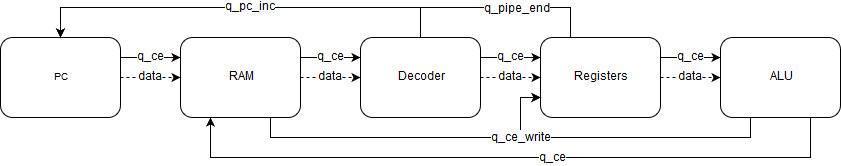
\includegraphics[width=1.0\textwidth]{prco_forward_pipe}
      \caption{The feed-forward pipeline interconnect diagram used by the \scname{} processor.}
       \label{fig:prco_forward_pipe}
\end{figure}

The pipeline structure is described in figure \ref{fig:prco_forward_pipe} (above). The general order of the modules is shown from left to right, but this can change due to the pipelines re-ordering functionality.

The Decoder module will decode instruction words from memory and will output appropriate signals containing the requirements of the instruction, such as requiring register write access, any ALU operation, and whether the instructions requires access to internal/external memory.
\newline\newline
To improve instruction performance, the decoder can also choose what modules are required and when they are called. For example, for the {\nameref{isa_movi}} (move immediate) instruction the Decoder will assign the following modules in the following order: ALU and Register write, resulting in a total of 5 stages (including PC, Fetch, and Decode). The last module in this pipeline, the Register write, will raise the \textit{q\_pipe\_end} signal indicating that the pipeline has finished and to start fetching the next instruction.

For the {\nameref{isa_nop}} instruction, the decoder identifies that the instruction requires no dependencies and will hence signal the \textit{q\_pc\_inc} signal resulting in only 3 pipeline stages.

For instructions that require RAM access, a typical pipeline order might look like: PC, Fetch, Decoder, Register Read, ALU, RAM, resulting in 6 stages being used.

\begin{figure}[H]
\begin{center}
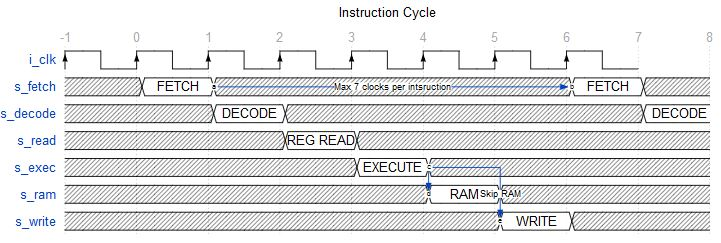
\includegraphics[scale=0.8]{td_instr}
\end{center}
\caption{\scname{} processor instruction cycle time diagram.}
\label{fig:dft_algorithm}
\end{figure}

\newpage
\subsection{Interrupts and Exceptions}\label{sect:interrupts}

\newpage
\section{\scname{} Instruction Set Architecture}
This section describes instructions available on the \scname{} processor.

The following instruction definitions use the following letters to describe values: X for any value; 0 for all zeros; 1 for all ones; Imm8 for unsigned 8-bit immediate; Simm5 for signed 5-bit immediate.

\subsection{Timings}\label{sect:isa_timings}
As the processor does not employ instruction pipelining techniques, but instead uses control signals to individually turn on sub-processes on the CPU. These sub-processes do not happen in parallel. 

For instructions that do not require a RAM read/write request, the RAM stage of the control sequence is skipped reducing the instruction cycle by 1 CPU clock for that instruction.

The fastest instruction in terms of CPU cycles is the NOP instruction. The greatest number of cycles for an instruction includes all RAM read/write request operations, such as the LW and SW instructions (see section \ref{sect:isa_general}).


\subsection{General Instructions} \label{sect:isa_general}
The term, general instruction, is given to instructions that are common to primitive operations such as arithmetic and comparison instructions.

\subsubsection{Instruction List}
\begin{table}[h]
    \begin{tabularx}{\textwidth}{|p{4cm}|c|c|c|c|X|}
    \hline
    Type 1 & 15-11 & 10-8 & 7-5 & 4-0 & Semantics \\
    \hline
    Type 2 & 15-11 & 10-8 & \multicolumn{2}{c|}{7-0} & Semantics \\
    \hline
    Type 3 & 15-11 & 10-8 & 7-5 & 4-2 & Semantics \\
    \specialrule{2pt}{-2pt}{0pt}
    
    NOP 	& 00000 & X & X & X & PC $<$= PC + 1 \\ \hline
    HALT	& X0000 & X & X & X & \\ \hline
    LW 		& 00001 & Rd & Ra & Simm5 & Rd $<$= RAM[Ra + Simm5] \\ \hline
    LW.L 	& X0001 & Rd & Ra & Simm5 & Rd $<$= (RAM[Ra + Simm5] \& 0xFF) \\ \hline
    SW 		& 00010 & Rd & Ra & Simm5 & RAM[Ra + Simm5] $<$= Rd \\ \hline
    SW.L	& X0010 & Rd & Ra & Simm5 & RAM[Ra + Simm5] $<$= Rd \& 0xFF \\ \hline
    MOV		& 00011 & Rd & Ra & X & Rd $<$= Ra \\ \hline
    MOVI 	& 00100 & Rd & \multicolumn{2}{c|}{Simm8}  & Rd $<$= Simm8 \\ \hline
    ADD 	& 01000 & Rd & Ra & X & Rd $<$= Rd + Ra \\ \hline
    ADDI 	& 01001 & Rd & \multicolumn{2}{c|}{Simm8}  & Rd $<$= Rd + Simm8 \\ \hline
    SUB		& 01010 & Rd & Ra & X & Rd $<$= Rd - Ra \\ \hline
    SUBI 	& 01011 & Rd & \multicolumn{2}{c|}{Simm8}  & Rd $<$= Rd - Simm8 \\ \hline
    JMP		& 01100 & Rd & \multicolumn{2}{c|}{X} & See {\nameref{isa_jmp}}. \\ \hline
    CMP		& 01101 & Rd & Ra & Rb & Set SR flags \\ \hline
    \end{tabularx}
    \caption{Number of respondants for treatment}
\end{table}

\subsubsection{NOP}\label{isa_nop}
\begin{description}[align=right,labelwidth=4cm]
\item [Description] The NOP instruction performs no action for 1 instruction cycle (see section  \ref{sect:isa_timings}).
\item [Assembly] NOP
\item [Pseudocode]
\item [Registers altered]
\item [Clock cycles] 2 (FETCH, DECODE)
\end{description}

\begin{table}[h]
\def\arraystretch{1.5}%  1 is the default, change whatever you need
    \begin{tabularx}{\textwidth}{|p{4cm}|X|}
    \hline
    15:11 & 10:0 \\
	\specialrule{2pt}{-2pt}{0pt}
	00000 & X
	\\ \hline
    \end{tabularx}
\end{table}


\subsubsection{LW - Load Word}\label{isa_lw}
\begin{description}[align=right,labelwidth=4cm]
\item [Description] Copies a 16-bit word from RAM to a register.
\item [Assembly] LW Rd, +4(Ra)
\item [Pseudocode] Rd $<=$ RAM[Ra + Simm5]
\item [Registers altered] Rd
\item [Clock cycles] 6 (FETCH, DECODE, READ, EXECUTE, RAM, WRITE)
\end{description}

\begin{table}[H]
\def\arraystretch{1.5}%  1 is the default, change whatever you need
    \begin{tabularx}{\textwidth}{|p{4cm}|p{2cm}|p{2cm}|X|}
    \hline
    15:11 & 10:8 & 7:5 & 4:0 \\
	\specialrule{2pt}{-2pt}{0pt}
	00001 & Rd & Ra & Simm5
	\\ \hline
    \end{tabularx}
\end{table}


\subsubsection{SW - Store Word}\label{isa_sw}
\begin{description}[align=right,labelwidth=4cm]
\item [Description] Copies a 16-bit from a register to RAM.
\item [Assembly] SW Rd, +4(Ra)
\item [Pseudocode] RAM[Ra+Simm5] $<=$ Rd
\item [Registers altered] None
\item [Clock cycles] 6 (FETCH, DECODE, READ, EXECUTE, RAM, WRITE)
\end{description}

\begin{table}[H]
\def\arraystretch{1.5}%  1 is the default, change whatever you need
    \begin{tabularx}{\textwidth}{|p{4cm}|p{2cm}|p{2cm}|X|}
    \hline
    15:11 & 10:8 & 7:5 & 4:0 \\
	\specialrule{2pt}{-2pt}{0pt}
	00001 & Rd & Ra & Simm5
	\\ \hline
    \end{tabularx}
\end{table}

\subsubsection{MOVR}
\begin{description}[align=right,labelwidth=4cm]
\item [Description] The MOVR instruction copies a 16-bit register value to another register.
\item [Assembly] MOVR \%Ra, \%Rd 
\item [Pseudocode] Rd $<=$ Ra
\item [Registers altered] Rd
\item [Clock cycles] 5 (FETCH, DECODE, READ, EXECUTE, WRITE)
\end{description}

\begin{table}[H]
\def\arraystretch{1.5}%  1 is the default, change whatever you need
    \begin{tabularx}{\textwidth}{|p{4cm}|p{2cm}|p{2cm}|X|}
    \hline
    15:11 & 10:8 & 7:5 & 4:0 \\
	\specialrule{2pt}{-2pt}{0pt}
	00011 & Rd & Ra & X
	\\ \hline
    \end{tabularx}
\end{table}

\subsubsection{MOVI}\label{isa_movi}
\begin{description}[align=right,labelwidth=4cm]
\item [Description] The MOVR instruction copies a 16-bit register value to another register.
\item [Assembly] MOVR \%Ra, \%Rd 
\item [Pseudocode] Rd $<=$ Ra
\item [Registers altered] Rd
\item [Clock cycles] 5 (FETCH, DECODE, READ, EXECUTE, WRITE)
\end{description}

\begin{table}[H]
\def\arraystretch{1.5}%  1 is the default, change whatever you need
    \begin{tabularx}{\textwidth}{|p{4cm}|p{3cm}|X|}
    \hline
    15:11 & 10:8 & 7:0 \\
	\specialrule{2pt}{-2pt}{0pt}
	00100 & Rd & Imm8
	\\ \hline
    \end{tabularx}
\end{table}


\subsubsection{ADD}
\begin{description}[align=right,labelwidth=4cm]
\item [Description] The ADD instruction adds an immediate value to a destination register, Rd.
\item [Assembly] ADDI \$255, \%Rd
\item [Pseudocode]Rd $<=$ Rd + Imm8
\item [Registers altered] Rd
\item [Clock cycles] 5 (FETCH, DECODE, READ, EXEC, WRITE)
\end{description}

\begin{table}[H]
\def\arraystretch{1.5}%  1 is the default, change whatever you need
    \begin{tabularx}{\textwidth}{|p{4cm}|p{2cm}|p{2cm}|X|}
    \hline
    15:11 & 10:8 & 7:5 & 4:0 \\
	\specialrule{2pt}{-2pt}{0pt}
	01000 & Rd & Ra & X
	\\ \hline
    \end{tabularx}
\end{table}

\subsubsection{ADDI}
\begin{description}[align=right,labelwidth=4cm]
\item [Description] The ADD instruction adds an immediate value to a destination register, Rd.
\item [Assembly] ADDI \$255, \%Rd
\item [Pseudocode]Rd $<=$ Rd + Imm8
\item [Registers altered] Rd
\item [Clock cycles] 5 (FETCH, DECODE, READ, EXEC, WRITE)
\end{description}

\begin{table}[H]
\def\arraystretch{1.5}%  1 is the default, change whatever you need
    \begin{tabularx}{\textwidth}{|p{4cm}|p{3cm}|X|}
    \hline
    15:11 & 10:8 & 7:0 \\
	\specialrule{2pt}{-2pt}{0pt}
	01001 & Rd & Imm8
	\\ \hline
    \end{tabularx}
\end{table}


\subsubsection{SUBI}
\begin{description}[align=right,labelwidth=4cm]
\item [Description] The SUB instruction subtracts an immediate value from a destination register, Rd.
\item [Assembly] SUBI \$255, \%Rd
\item [Pseudocode]Rd $<=$ Rd - Imm8
\item [Registers altered] Rd
\item [Clock cycles] 5 (FETCH, DECODE, READ, EXEC, WRITE)
\end{description}

\begin{table}[H]
\def\arraystretch{1.5}%  1 is the default, change whatever you need
    \begin{tabularx}{\textwidth}{|p{4cm}|p{3cm}|X|}
    \hline
    15:11 & 10:8 & 7:0 \\
	\specialrule{2pt}{-2pt}{0pt}
	01001 & Rd & Imm8
	\\ \hline
    \end{tabularx}
\end{table}


\subsubsection{CMP}
\begin{description}[align=right,labelwidth=4cm]
\item [Description] Sets register, Rd, to the value of Ra - Rb.
\item [Assembly] CMP Rd, Ra, Rb
\item [Pseudocode]Rd $<=$ CMP(Ra, Rb)
\item [Registers altered] Rd
\item [Clock cycles] 5 (FETCH, DECODE, READ, EXEC, WRITE)
\item [Note] Rd should be set to SR ({\nameref{sect:sr}}) as the {\nameref{isa_jmp}} instruction operates on the SR register.
\end{description}

\begin{table}[H]
\def\arraystretch{1.5}%  1 is the default, change whatever you need
    \begin{tabularx}{\textwidth}{|p{4cm}|p{2cm}|p{2cm}|p{2cm}|X|}
    \hline
    15:12 & 11:9 & 8:6 & 5:3 & 2:0 \\
	\specialrule{2pt}{-2pt}{0pt}
	0003 & Rd & Ra & Rb & X
	\\ \hline
    \end{tabularx}
\end{table}

\newpage
\subsubsection{JMP}\label{isa_jmp}
\begin{description}[align=right,labelwidth=4cm]
\item [Description] Jumps the {\nameref{sect:pc}} if the condition is met within the {\nameref{sect:sr}} register.
\item [Assembly] JMP Rd, Imm8
\item [Pseudocode] {\nameref{sect:pc}} $<=$ Rd if ({\nameref{sect:sr}} \& Imm8).
\item [Registers altered] None
\item [Clock cycles] 5 (FETCH, DECODE, READ, EXEC, BRANCH)
\end{description}

\begin{table}[H]
\def\arraystretch{1.5}%  1 is the default, change whatever you need
    \begin{tabularx}{\textwidth}{|p{4cm}|p{3cm}|X|}
    \hline
    15:11 & 10:8 & 7:0 \\
	\specialrule{2pt}{-2pt}{0pt}
	01100 & Rd & Imm8
	\\ \hline
    \end{tabularx}
\end{table}
An 8 bit immediate (7-0) can be set in the JMP instruction to create conditional jumps.

\begin{table}[h]
	\def\arraystretch{1.5}%  1 is the default, change whatever you need
    \begin{tabularx}{\textwidth}{|c|c|c|c|c|X|X|}
    \hline
    & 15-11 & 10-8 & \multicolumn{2}{c|}{7-0} & Semantics & Status Register \\
    \specialrule{2pt}{-2pt}{0pt}
    JMP		& 01100 & Rd & \multicolumn{2}{c|}{0000 0000} & Unconditional Jump & Any\\ \hline
    JE		& 01100 & Rd & \multicolumn{2}{c|}{0000 0001} & Jump Equal & ZF=1\\ \hline
    JNE		& 01100 & Rd & \multicolumn{2}{c|}{0000 0010} & Jump Not Equal & ZF=0\\ \hline
    JG	& 01100 & Rd & \multicolumn{2}{c|}{0000 0011} & Jump Greater Than & ZF=0 and SF=OF\\ \hline
    JGE		& 01100 & Rd & \multicolumn{2}{c|}{0000 0100} & Jump Greater Than or Equal & SF=OF\\ \hline
    JL		& 01100 & Rd & \multicolumn{2}{c|}{0000 0101} & Jump Less Than & SF$<>$OF\\ \hline
    JLE		& 01100 & Rd & \multicolumn{2}{c|}{0000 0110} & Jump Less Than or Equal & ZF=1 or SF$<>$OF\\ \hline
    JS		& 01100 & Rd & \multicolumn{2}{c|}{0000 0111} & Jump Signed & SF=1\\ \hline
    JNS		& 01100 & Rd & \multicolumn{2}{c|}{0000 1000} & Jump Not Signed & SF=0 \\ \hline
    \end{tabularx}
    \caption{Conditional jump immediate bits}
\end{table}


\subsection{Special Instructions}

\newpage
\section{Compiler}
\subsection{Features}
\subsection{Usage}
The compiler is invoked using the libprco/cli executable.

\subsection{Grammar}
\subsection{Code Generation}



\newpage
\bibliography{prco304} 
\end{document}